\chapter{Теоретический раздел}

\section{Алгоритм SHA1}

На рисунке \ref{img:sha1p} представлена общая схема реализации алгоритма хеширования SHA1.

\begin{table}[H]
	\centering
	\begin{tabular}{p{1\linewidth}}
		\centering
		\includegraphics[width=0.5\linewidth]{assets/sha1}
		\captionof{figure}{Общая схема реализации алгоритма хеширования SHA1}
		\label{img:sha1p}
	\end{tabular}
\end{table}

\section{Алгоритм RSA}
На рисунках \ref{img:rsa}--\ref{img:rsa_keygen} представлена общая схема реализации алгоритма шифрования RSA.

\begin{table}[H]
	\centering
	\begin{tabular}{p{1\linewidth}}
		\centering
		\includegraphics[width=1.0\linewidth]{assets/rsa.png}
		\captionof{figure}{Общая схема реализации алгоритма шифрования RSA}
		\label{img:rsa}
	\end{tabular}
\end{table}

\begin{table}[H]
	\centering
	\begin{tabular}{p{1\linewidth}}
		\centering
		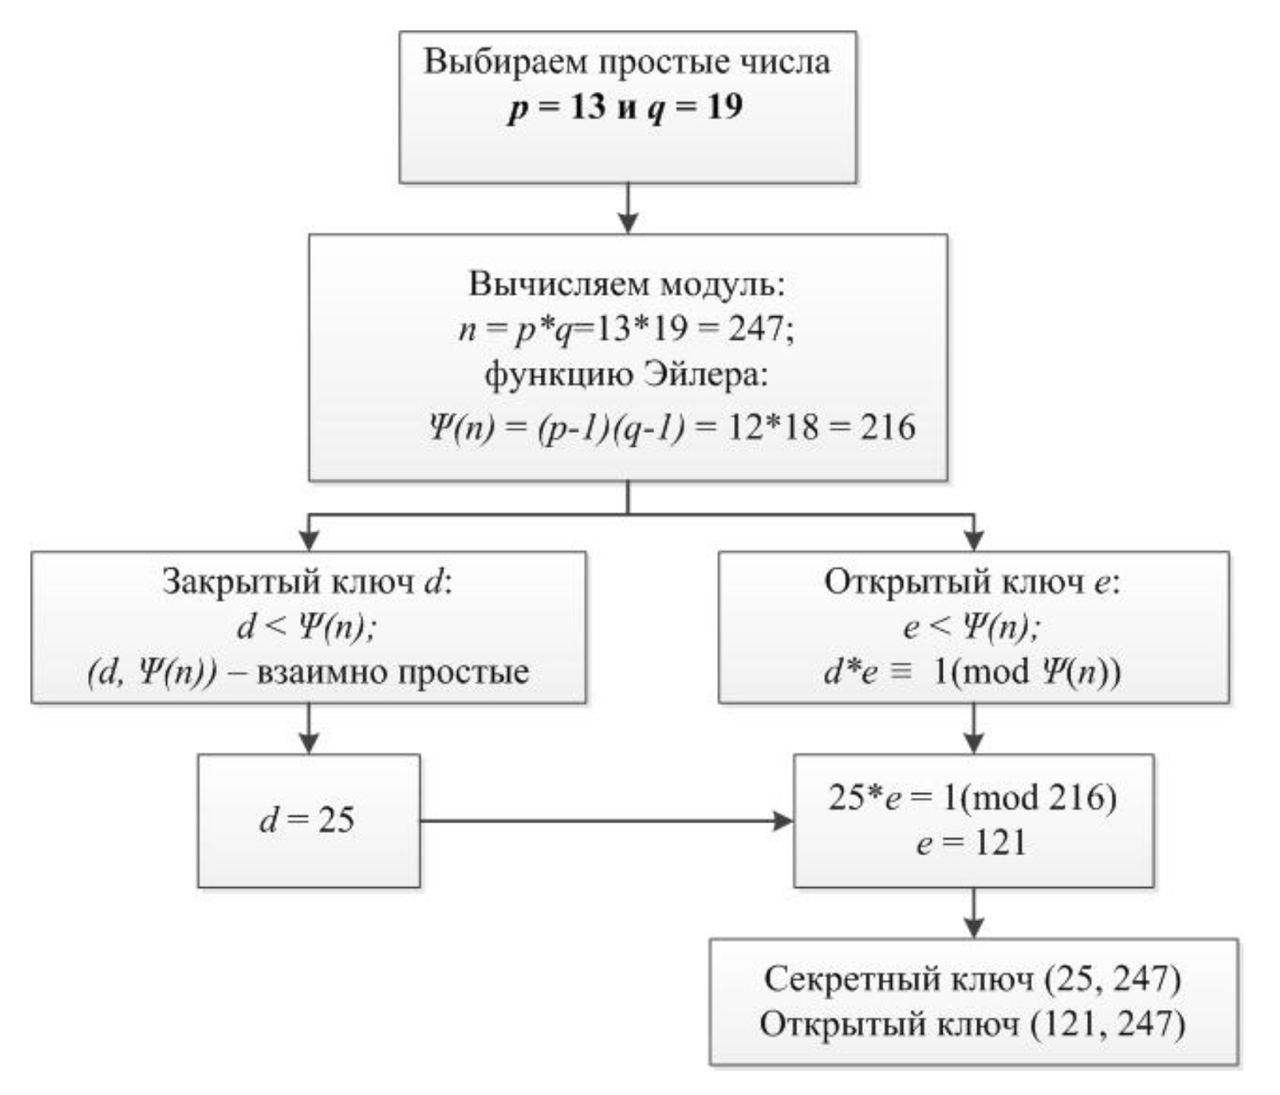
\includegraphics[width=1.0\linewidth]{assets/rsa_keygen.jpeg}
		\captionof{figure}{Общая схема реализации алгоритма генерации ключей RSA}
		\label{img:rsa_keygen}
	\end{tabular}
\end{table}

\newpage

\section{Цифровая подпись}

На рисунках \ref{img:sign}--\ref{img:check} представлена общая схема алгоритма электронной подписи и проверки электронной подписи.

\begin{table}[H]
	\centering
	\begin{tabular}{p{1\linewidth}}
		\centering
		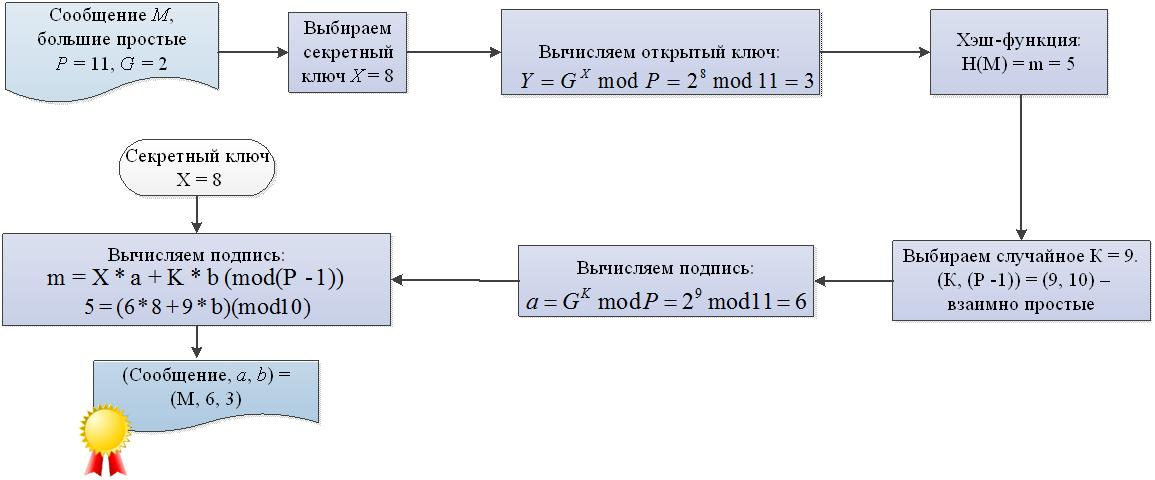
\includegraphics[width=0.75\linewidth]{assets/sign.jpeg}
		\captionof{figure}{Общая схема алгоритма электронной подписи}
		\label{img:sign}
	\end{tabular}
\end{table}

\begin{table}[H]
	\centering
	\begin{tabular}{p{1\linewidth}}
		\centering
		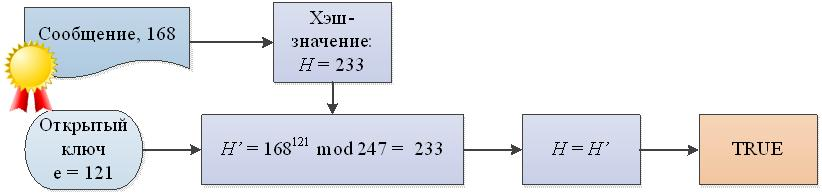
\includegraphics[width=0.75\linewidth]{assets/check}
		\captionof{figure}{Общая схема алгоритма проверки электронной подписи}
		\label{img:check}
	\end{tabular}
\end{table}
